\chapter{Microservizi}

Un'architettura a microservizi è una variante dell'architettura \textit{Service oriented} che prevede di strutturare un'applicazione come un insieme di moduli disaccoppiati tra loro, indipendentemente rilasciabili, manutenibili e testabili.\\
I servizi possono comunicare tra loro tramite protocolli di vario tipo, sia sincroni che asincroni.

\section{Scalabilità}
Un'applicazione enterprise nasce naturalmente come costituita da un singolo blocco in esecuzione su di un dispositivo (fisico o virtuale).\\
I sistemi di questo tipo hanno successo quando, una volta rilasciato il software, il numero di utilizzatori rimane limitato e la manutenzione non introduce troppe nuove funzionalità.
Altrimenti, per evitare un deterioramento delle performance o eventuali fallimenti, è necessario affrontare il tema della scalabilità quando il sistema è già online, nel caso questo non sia già stato fatto in fase di progettazione.

\subsection{The Scale Cube}
In figura \ref{fig:scale_cube}\cite{the_art_of_scalability} è mostrato uno dei possibili modelli su cui è possibile lavorare per ottenere un'applicazione scalabile.
In particolare in questa rappresentazione è possibile muoversi lungo i tre assi cartesiani per ottenere scalabilità in modi diversi:

\begin{figure}[h]
	\centering
	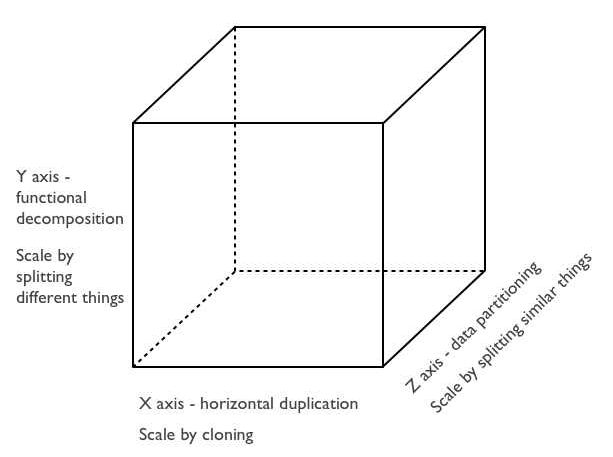
\includegraphics[scale=0.5]{img/scale_cube}
	\caption{Modulo ad architettura ports and adapters}
	\label{fig:scale_cube}
\end{figure}


\subsubsection{Asse X}
Scalare un sistema \textit{sull'asse X} significa avere più repliche della stessa applicazione in produzione; questo permette di gestire un maggior numero di richieste al secondo, eliminare i \textit{single point of failure} e non richiede grandi costi aggiuntivi di progettazione o rifattorizzazione.
Gli accessi sono gestiti da un \textit{load balancer} che avrà la responsabilità di effettuare un inoltro all'istanza più appropriata in base a vari criteri, quali zona geografica, presenza di guasti, carico di lavoro ecc...
\'E quindi possibile scegliere sistemi che operano con protocolli a vari livelli, come applicazione, trasporto o rete.
Ogni nodo potenzialmente può accedere a tutti i dati, quindi questo tipo di organizzazione non migliora i requisiti di memoria per istanza.

\subsubsection{Asse Z}
Scalare un sistema \textit{sull'asse Z} significa avere lo stesso codice replicato su più server come nel caso X, ma in questo caso ogni copia è responsabile di un sottoinsieme dei dati: il load balancer dovrà quindi inoltrare le richieste in base al contenuto di esse, operando quindi a livello applicazione.\\
Questa scelta permette di ridurre le risorse necessarie ad ogni istanza, compresa la quantità di storage o di memoria riservata alla cache.

\subsubsection{Asse Y}
Scalare un sistema \textit{sull'asse Y} significa effettuare una partizione del software per dati e/o funzionalità, partendo da un'analisi di casi d'uso e modello di dominio.\\
Si ottengono così più istanze uniche, ognuna con le proprie responsabilità ed il proprio modello di dominio.
La complessità del software viene quindi ridotta, le risorse ottimizzate la manutenibilità migliorata.\\
Questo approccio incide maggiormente sulla fase di progettazione, mentre un modo rapido per implementare questa strategia su un sistema preesistente può essere quello di replicare l'applicazione per intero come nei casi precedente e delegare ad ogni replica un particolare compito sulla base delle divisioni individuate per mezzo di un load balancer di livello applicazione.

\section{Partizionamento in microservizi}
Progettare un sistema a microservizi non è semplice quanto progettarne uno monolitico/service oriented tradizionale: difficilmente infatti un software nasce già partizionato, e a causa delle diverse complessità che questo approccio si porta dietro non è consigliabile utilizzarlo come prima carta.\\
Solitamente si sceglie di passare a tale architettura in un secondo momento, per esempio dopo molti interventi di manutenzione, quando il codice inizia ad essere troppo ampio e complesso.\cite{microservices_architecture}
In termini di scalabilità l'adottare i microservizi riguarda l'asse Y dello \textit{Scale Cube}.

Alcuni dei vantaggi principali del passare ad una architettura a microservizi sono:
\begin{itemize}
	\item Maggior facilità di manutenzione e testing.
	\item Maggiore indipendenza dei team di lavoro grazie al disaccoppiamento dei servizi.
	\item Messa in produzione indipendente.
	\item Team di sviluppo di piccole dimensioni.
\end{itemize}

\subsection{Saga}
Con il termine \textit{saga} si intende un insieme di piccole transazioni locali autoconsistenti.\\
Il coordinamento avviene in modo distribuito: ogni servizio lancerà eventi in caso di completamento o fallimento di una transazione; questi saranno quindi interpretati dagli altri moduli.\\
\'E possibile delegare le opzioni di coordinamento ad oggetti appositi.

https://microservices.io/patterns/data/saga.html

\section{Caratteristiche di un microservizio}

Temi ricorrenti quando si parla di microservizi sono quelli riguardanti la dimensione che un servizio deve avere, il numero di responsabilità, l'integrità delle informazioni ecc...\\
La linea guida principale da seguire è quella di fare in modo che i servizi siano il più possibile indipendenti tra loro, favorendo coesione, evitando un eccessivo accoppiamento.\\
Un servizio per essere tale dev'essere rilasciabile in modo indipendente dagli altri: esso infatti è l'unità minima dell'architettura. Ognuno può potenzialmente utilizzare la propria tecnologia, cosa che favorisce l'evoluzione ed evita che il software nel tempo resti legato ad una tecnologia datata.\\
Il partizionamento del monolite deve portare ad avere un certo numero di servizi disaccoppiati ma coesi: occorre studiare bene quali siano i giusti confini lungo cui tagliare il software, in modo che i nodi possano lavorare in indipendenza, ognuno con le proprie responsabilità.